% Evidence-to-policy diagram: Truth -> Research -> Policy Analysis ->
% Policy Makers -> Support/Oppose. The single source for every project that
% uses it; build with ./build.sh, which writes both variants to out/.
%   web   : all circles 2.4cm (personal website)
%   paper : Research circle 2.0cm (JMP paper, Registration-Tips deck)

\documentclass[border=10pt,tikz]{standalone}
\usepackage{tikz}
\usetikzlibrary{positioning,shapes.geometric}
\pdftrailerid{}

% Variant switch: build.sh defines \paperversion for the paper/slide copy,
% in which the Research circle is smaller (2.0cm). Web: every circle 2.4cm.
\ifdefined\paperversion\def\researchsize{2.0cm}\else\def\researchsize{2.4cm}\fi

\begin{document}
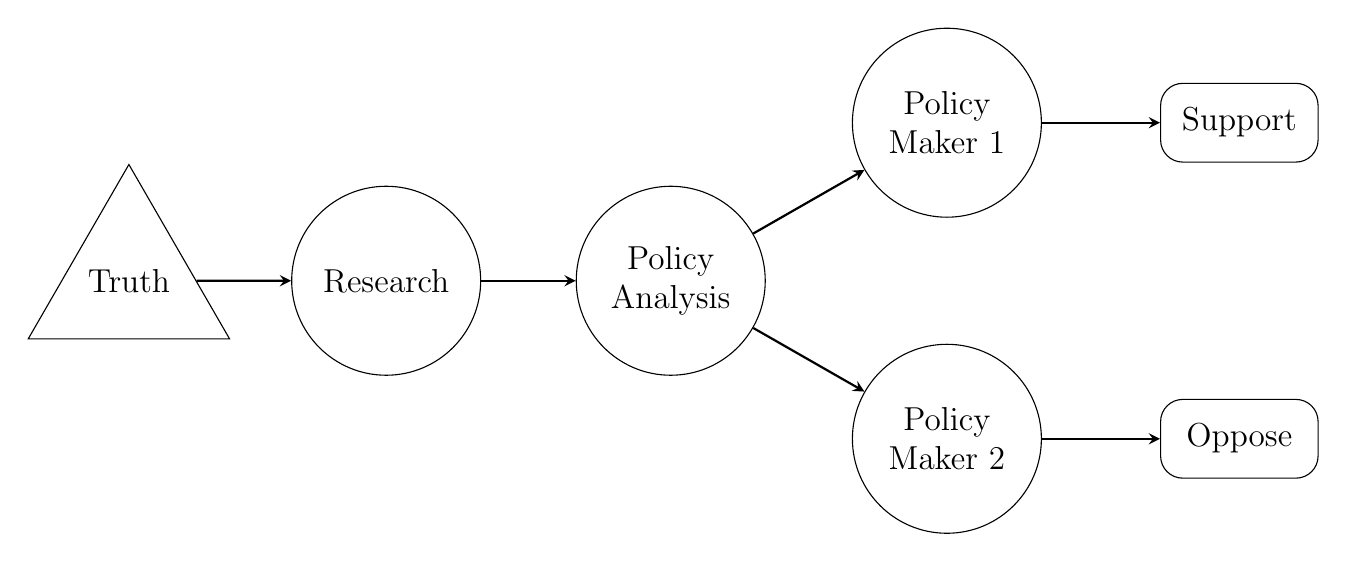
\begin{tikzpicture}[
  every node/.style={font=\large},
  bigcirc/.style={circle, draw, minimum size=2.4cm, align=center, inner sep=2pt},
  tri/.style={regular polygon, regular polygon sides=3, draw,
              minimum size=2.5cm, align=center, inner sep=0pt},
  rrect/.style={rectangle, rounded corners=8pt, draw, minimum width=2cm,
                minimum height=1cm, align=center},
  arr/.style={-stealth, thick}
]

\node[tri]                                        (T)   {Truth};
\node[bigcirc, minimum size=\researchsize, right=1.2cm of T] (R) {Research};
\node[bigcirc, right=1.2cm of R]                  (PA)  {Policy\\Analysis};
\node[bigcirc, above right=0.3cm and 1.8cm of PA] (PM1) {Policy\\Maker 1};
\node[bigcirc, below right=0.3cm and 1.8cm of PA] (PM2) {Policy\\Maker 2};
\node[rrect,   right=1.5cm of PM1]                (S)   {Support};
\node[rrect,   right=1.5cm of PM2]                (O)   {Oppose};

\draw[arr] (T)   -- (R);
\draw[arr] (R)   -- (PA);
\draw[arr] (PA)  -- (PM1);
\draw[arr] (PA)  -- (PM2);
\draw[arr] (PM1) -- (S);
\draw[arr] (PM2) -- (O);

\end{tikzpicture}
\end{document}
